\documentclass[a4paper,twoside,12pt,openright]{report}

%% Language %%%%%%%%%%%%%%%%%%%%%%%%%%%%%%%%%%%%%%%%%%%%%%%%%
\usepackage[francais]{babel}
\usepackage[utf8]{inputenc}
\usepackage[T1]{fontenc}
\usepackage{lmodern} 
\usepackage{hyperref}
\usepackage{tabto}

%% Packages for Graphics & Figures %%%%%%%%%%%%%%%%%%%%%%%%%%
\usepackage{graphicx} 

%% Math Packages %%%%%%%%%%%%%%%%%%%%%%%%%%%%%%%%%%%%%%%%%%%%
\usepackage{amsmath}
\usepackage{amsthm}
\usepackage{amsfonts}
\usepackage{fullpage}

\setlength{\parindent}{0cm}
\setlength{\parskip}{1ex plus 0.5ex minus 0.2ex}
\newcommand{\hsp}{\hspace{20pt}}
\newcommand{\HRule}{\rule{\linewidth}{0.5mm}}
%%%%%%%%%%%%%%%%%%%%%%%%%%%%%%%%%%%%%%%%%%%%%%%%%%%%%%%%%%%%%
%% DOCUMENT
%%%%%%%%%%%%%%%%%%%%%%%%%%%%%%%%%%%%%%%%%%%%%%%%%%%%%%%%%%%%%
\begin{document}
\begin{titlepage}
  \begin{sffamily}
  \begin{center}

    \textsc{\LARGE MASTER MIAGE 2ème année \linebreak Université Paris Nanterre}\\[2cm]

    \textsc{\Large Mémoire de fin d’études présenté pour l’obtention du grade de master}\\[1.5cm]

    \HRule \\[0.4cm]
    { \huge \bfseries Comment les flots de contrôle peuvent-ils nous permettre de faire du refactoring de code en Java. \\[0.4cm] }

    \HRule \\[2cm]
    
\includegraphics[scale=0.40]{image/univ.jpg}
    \hspace{2cm}
    
    \vfill
  \begin{minipage}{0.4\textwidth}
      \begin{flushleft} \large
        \textsc{Présenté par :}\\ \textsc{Thibault Sartre}\\
      \end{flushleft}
    \end{minipage}
    \begin{minipage}{0.4\textwidth}
      \begin{flushright} \large
        \textsc{Tuteur :}\\ \textsc{Mcf. Emmanuel Hyon}\\
      \end{flushright}
    \end{minipage}
    \vfill
    {\large Septembre 2018 — Juillet 2019}
  \end{center}
  \end{sffamily}
\end{titlepage}
\renewcommand{\contentsname}{Sommaire}
\tableofcontents{}
\chapter{Contexte}
\section{Introduction}
Le refactoring est une activité d'ingénierie logiciel consistant à modifier le code source d'une application de manière à améliorer sa qualité sans altérer son comportement vis-à-vis des utilisateurs.
L'objectif du refactoring est de réduire les coûts de maintenance et de pérenniser les investissements tout au long du cycle de vie du logiciel en se concentrant sur la maintenabilité et l'évolutivité.\cite{ref1}\\
"With refactoring you can take a bad design, chaos even, and rework it into well-designed code."\cite{ref2}\\
Le refactoring permet donc de passer d'un code possédant de mauvaise base à un code propre.\\
Un bon refactoring doit pouvoir améliorer la qualité d'un code tout en gardant son fonctionnement du point de vue de l'utilisateur. Concernant la partie des tests, tout les tests qui fonctionnaient avant le refactoring se doivent d'être fonctionnels après.\\
Dans ce mémoire, nous allons analyser différentes techniques de refactoring. Puis nous allons étudier les outils de refactoring existant ainsi que les graphes de flot de contrôle.\\ Enfin on étudiera s'il est possible de faire du refactoring à l'aide des flots de contrôle pour le langage Java.\\
Ce sujet est intéressant et actuel car il faut commencer à ce soucier du code que l'on produit car plus l'on avance dans le temps plus les programmes sont lourds et contiennent de lignes de code. Avec la puissance des ordinateurs actuels, la plus part des développeurs ne prennent plus le temps d'écrire des codes de qualité car la machine sera de toute façon assez rapide pour compenser un code de mauvaise qualité.\cite{ref4}\\
Avec le temps, la relecture et la modification de code sera difficile avec les programmes qui deviennent de plus en plus gros.\cite{ref4}\\
Pour essayer de diminuer cette quantité de travail à l'avenir, il faut commencer à produire du code de qualité et bien structuré. Concernant les codes déjà existant il faudra donc faire du refactoring de code. Or le refactoring peut-être long selon la qualité des projets que l'on traite. Il serait donc intéressant et très utile d'avoir un programme permettant d'automatiser des parties de refactoring pour permettre de gagner du temps précieux. 
Ce mémoire a pour but de fournir une solution qui permettrais de faire du refactoring de code facilement pour gagner du temps tout en produisant du code de qualité.\cite{ref3}

\chapter{Les différents type de refactoring}
\section{Pattern de méthode composée}
L'un des grands ennemie des développeurs est de faire des méthodes trop longue qui sont difficilement compréhensible.
Une grande partie du refactoring est donc consacrée à la composition correcte des méthodes.\cite{ref5}\\

L'objectif de ce type de refactoring est de :\\
- rendre les méthodes facilement compréhensible.\\
- simplifier les méthodes en les brisants en plusieurs méthodes plus petites.\\
- supprimer la duplication de code.\\
- nommer proprement les variables, méthodes et paramètres pour comprendre leurs utilités au premier coup d'œil.\\
- pouvoir faire des tests plus facilement car les morceaux de méthodes peuvent être testés individuellement.\cite{ref6}

\newpage

\subsection{Extraction de méthode}
\paragraph{Présentation :} 
La technique d'extraction de méthode permet comme son nom l'indique, d'extraire des méthodes (ou fonction) du code. Car plus il y a de ligne dans une méthode plus il est difficile de comprendre ce que fait la méthode.\\
Il faut donc lorsque c'est possible extraire du code pour former d'autre méthode et simplifier le code.
\begin{center}
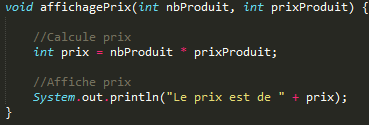
\includegraphics[scale=1]{Image/Extraction_Methode.png}\\
\itshape{Avant extraction de méthode}
\end{center}

\paragraph{Exemple :} 
Au dessus nous avons une méthode qui va afficher le prix d'un produit tout en calculant elle même le prix.\\
Si l'on applique l'extraction de méthode, on va obtenir l'exemple du bas, c'est à dire extraire la méthode de calcule du prix car on en aura surement besoin ailleurs. On remplace donc la calcule du prix dans la méthode affichagePrix par un appel à la méthode calculePrix.\\
\begin{center}
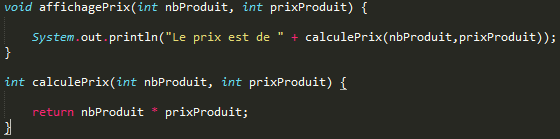
\includegraphics[scale=1]{Image/Extraction_Methode2.png}\\
\itshape{Après extraction de méthode}
\end{center}
\paragraph{Bénéfices :}
Pour que cette technique de refactoring soit la plus efficace, il faut absolument nommer ses méthodes et les paramètres de manière à comprendre très facilement qu'elle est sont but et que représente les paramètres. Le code est donc bien plus lisible.\\\\
A l'aide de cette méthode, on évite la duplication de code. Puisque dans l'exemple on aurait pu vouloir calculer le prix d'un produit dans une autre méthode, avec le code au dessus on aurait dupliqué le code pour calculer le prix d'un produit.\\\\
L'extraction de méthode nous permet aussi d'isoler les parties indépendantes du code. Cela est pratique lorsque l'on cherche un potentiel bug, on peut plus facilement tester toutes les méthodes du codes car elles sont toutes isolées les une des autres.

\paragraph{Technique inverse :}
La technique de refactoring Inline Method est l'exact opposé de l'extraction de méthode. Cette technique consiste à supprimé les méthodes jugées inutile qui sont très courtes ou qui sont plus facilement compréhensible par le code à l'intérieure de la méthode que par son nom. Cela à pour seul but de simplifier le code en diminuant le nombre de méthode dans le code.

\subsection{Extraction de variable}
\paragraph{Présentation :}
La technique d'extraction de variable permet de créer des variables claires qui nous permet de rendre des expressions complexe plus compréhensible.
Elle peut s'appliquer, par exemple, sur les conditions de if ou aussi des expressions arithmétiques sans résultats intermédiaires.

\begin{center}
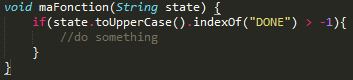
\includegraphics[scale=1]{Image/Extraction_Variable.png}\\
\itshape{Avant extraction de variable}
\end{center}

\paragraph{Exemple :}
Au dessus, nous pouvons voir une fonction qui va faire quelque chose si l'état est done.
Si l'on applique l'extraction de variable, on obtient une variable isDone qui contient un boolean. Cette méthode nous permet de passer d'un code qui contient une expression peu lisible à un code avec une variable explicite.

\begin{center}
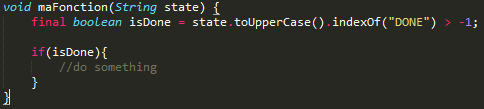
\includegraphics[scale=1]{Image/Extraction_Variable2.png}\\
\itshape{Après extraction de variable}
\end{center}

\paragraph{Bénéfices :}
Pour que le résultat de cette méthode soit optimal, il faut nommer efficacement les variables créées pour  qu'elles soient le plus lisible possible. Cela va permettre de produire un code plus lisible et qui contiendra moins de long commentaire pour expliquer les longues expressions.

\paragraph{Inconvénient :}
Le code va contenir beaucoup de variable mais cela est dérisoire comparé à la lisibilité du code qui est nettement améliorée.

\paragraph{Technique inverse :}
La technique Inline Temp va permettre de supprimer les variables superflue qui contienne uniquement le résultat d'une opération simple qui va être utilisé une seul fois. Cette technique n'a pas de vrai bénéfice dans cette état, en revanche elle peut être couplé avec la technique suivante.

\subsection{Remplacement des temporaires avec des méthodes}
\paragraph{Présentation :}
Le remplacement des temporaires avec des méthodes va comme son nom l'indique, remplacer des variables temporaires par le résultat de méthode. On va extraire le code des variables temporaire avec la technique Inline method puis les placer dans des méthodes.

\begin{center}
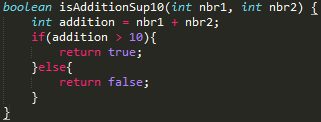
\includegraphics[scale=1]{Image/Remplacement_Temp_Methode.png}\\
\itshape{Avant remplacement du temporaire}
\end{center}

\paragraph{Exemple :}
Au dessus, nous pouvons voir que l'addition des deux paramètre est stocké dans une variable temporaire. Après le refactoring, la variable temporaire disparait et on obtient une méthode qui va s'occuper de faire l'addition à la place.

\begin{center}
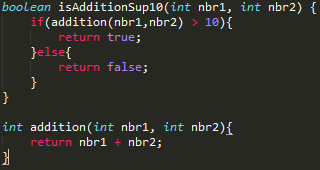
\includegraphics[scale=1]{Image/Remplacement_Temp_Methode2.png}\\
\itshape{Après remplacement du temporaire}
\end{center}

\paragraph{Bénéfices :}
Le code est plus compréhensible grâce au nom de la méthode qui est explicite.\\
Si j'ai besoin plus tard dans mon code de faire une addition, j'ai une méthode que je peux réutiliser.

\newpage

\subsection{Diviser les variables temporaires}
\paragraph{Présentation :}
Parfois dans notre code, nous déclarons une variable temporaire où nous stockons un résultat quelconque. Puis plus tard, nous réutilisons cette même variable pour stocker un tout autre résultat n'ayant aucun rapport.
Cette technique a pour but de ne plus utiliser la même variable temporaire pour faire différentes choses et de nommer proprement chaque variable temporaire.

\begin{center}
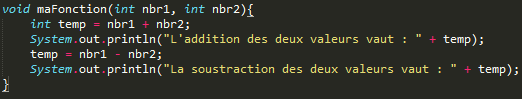
\includegraphics[scale=1]{Image/Diviser_Temp.png}\\
\itshape{Avant division}
\end{center}

\paragraph{Exemple :}
On peut voir au dessus que je réutilise la variable temp pour faire à la fois une addition et une soustraction. Après le refactoring on obtient deux variable proprement nommées addition et soustraction.

\begin{center}
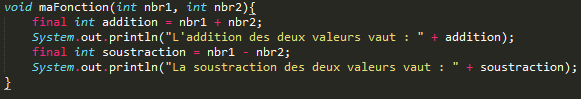
\includegraphics[scale=1]{Image/Diviser_Temp2.png}\\
\itshape{Après division}
\end{center}

\paragraph{Bénéfices :}
Le fait d'avoir chaque variable, méthode ou n'importe quelle composant qui a un unique but ou une responsabilité permet de faciliter grandement la maintenance du code. Puisque on peut modifier des parties du code sans que ça affecte une autre partie.\\
Cela permet aussi une meilleure relecture du code car on supprime les variables nommées temp ou value pour donner des noms facilement compréhensible.

\subsection{Supprimer les assignations aux paramètres}
\paragraph{Présentation :}
Ici le problème est semblable à celui de la division des variables temporaires, si on a un paramètre, on ne doit pas lui affecter d'autre valeur car cela modifie ce que représente le paramètre et on peut se perdre dans le code car on ne sait plus ce que contient ce paramètre.\\
Il vaut donc mieux déclarer une variable local plutôt que de modifier le paramètre.

\paragraph{Bénéfices :}
Comme dit plus haut, chaque éléments à une unique responsabilité et la maintenance du code est plus simple.  

\subsection{Remplacement de méthode par des objets}
\paragraph{Présentation :}
Il nous arrive d'écrire des méthodes très longues qui possèdent beaucoup de variable qui sont extrêmement liées entre elles. On peut avec le refactoring créer une nouvelle classe qui va contenir la méthode ainsi que les anciennes variables locales en variable de classe.

\begin{center}
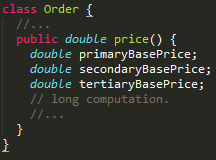
\includegraphics[scale=1]{Image/MethodeToObjet.png}\\
\itshape{Avant remplacement par l'objet \cite{ref5}}
\end{center}

\begin{center}
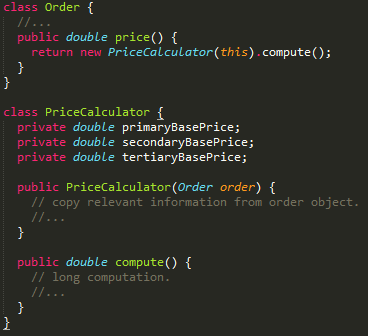
\includegraphics[scale=1]{Image/MethodeToObjet2.png}\\
\itshape{Après remplacement par l'objet \cite{ref5}}
\end{center}

\paragraph{Bénéfices :}
L'isolation d'une méthode longue dans sa propre classe permet d'empêcher le fait prenne de l'ampleur.\\
On peut aussi scinder cette méthode en sous-méthode sans "polluer" la classe d'origine avec des méthodes utilitaires.

\paragraph{Inconvénient :}
Cette méthode de refactoring nous fait créer une nouvelle classe et cela augmente la complexité global du programme.

\newpage

\section{Déplacement des fonctionnalités entre les objets}
Lorsque l'on code beaucoup de fonctionnalités dans un même programme, il arrive qu'au bout d'un moment, on se rendent compte que , par exemple, on a placé une fonctionnalité dans la mauvaise classe et qu'on ne sache pas comment faire pour la déplacer sans risquer de casser tout le code.\\
Or les méthodes de refactoring qui vont suivre seront du type à permettre le déplacement de fonctionnalités entre des classes en toute sécurité.


\subsection{Déplacement de méthode}
\paragraph{Présentation :}
Il se peut qu'à un instant t, vous vouliez déplacer une méthode dans un autre classe car cela vous arrange ou car cela aurait plus de sens. Dans ce cas la, on peut utiliser le refactoring pour déplacer cette méthode vers l'autre classe en toute sécurité.

\paragraph{Comment faire :}
Il faut commencer par regarder toutes les variables qui sont présente dans la classe et que la méthode utilise. Si c'est variable ne sont utilisé que par la méthode à déplacer, il faut les déplacer dans la nouvelle classe aussi.\\
En revanche si ces variables sont utilisées par d'autre méthode il est conseillé de déplacer aussi ces méthodes vers la nouvelle classe.
Ensuite, il faut s'assurer que toutes ces méthodes ne soit pas déclarer dans une classe mère ou fille.\\
Si toutes ces conditions sont réunis, on peut déclarer la ou les méthodes dans la nouvelle classe puis définir une méthode dans l'ancienne classe qui va appeler la nouvelle méthode.

\paragraph{Bénéfices :}
Cette méthode de refactoring nous permet d'obtenir une meilleure cohérence interne dans les classes.

\subsection{Extraction de classe}
\paragraph{Présentation :}
Il est possible, lorsque l'on développe quelque chose, de créer un classe qui en réalité fait le travail de deux classes. Il vaut mieux changer ça rapidement car cela risque d'empirer et d'obtenir une classe illisible. On peut alors appliquer une technique de refactoring pour extraire une classe d'une autre.

\begin{center}
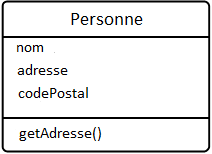
\includegraphics[scale=1]{Image/Extraction_Classe.png}\\
\itshape{Avant extraction de la classe}
\end{center}

\begin{center}
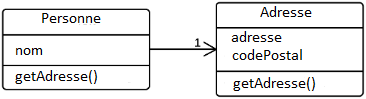
\includegraphics[scale=1]{Image/Extraction_Classe2.png}\\
\itshape{Après extraction de la classe}
\end{center}

\paragraph{Comment faire :}
Il faut d'abord créer la nouvelle classe ainsi qu'une relation entre l'ancienne et la nouvelle classe.\\
Ensuite, il faut utiliser les méthodes de refactoring "Déplacement de méthode" et "Déplacement de variable" pour toutes les variables et méthodes à déplacer.

\paragraph{Bénéfices :}
Cette méthode de refactoring permet de respecter le principe de responsabilité unique.
Les classes respectant ce principe sont plus fiable et tolérante aux changements puisque si une classe peut faire plusieurs choses, la modification d'une fonctionnalité de la classe peut casser une autre fonctionnalité.

\paragraph{Technique inverse :}
La technique inverse consiste à supprimer les classes qui ont peut d'utilités. Cela permet de libérer de la mémoire.

\subsection{Cacher la délégation}
\paragraph{Présentation :}
Nous sommes dans le cas où une structure permet à un client d'appeler une méthode d'un objet A qui lui renvoie un objet B pour ensuite appeler une méthode de l'objet B pour obtenir l'information souhaitées. On obtient une chaîne d'appel or si l'on veut changer quelque chose à la relation entre A et B, cela aura pour conséquence de changer la chaîne d'appel côté client.\\
Pour éviter ça, il est préférable de cacher la délégation au yeux du client à l'aide de refactoring.

\begin{center}
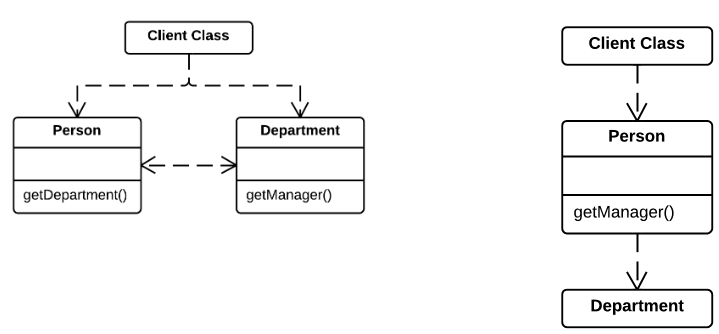
\includegraphics[scale=0.7]{Image/Cacher_Delegation.png}\\
\itshape{Avant/Après le refactoring \cite{ref5}}
\end{center}

\paragraph{Comment faire :}
Il faut commencer par créer dans la classe serveur (la classe dont le client à un access direct) les mêmes méthodes qui sont dans la classe déléguer (la classe qui contient les informations dont le client à besoin).\\
Ensuite, il faut changer le code client pour qu'il appel la méthode de la classe serveur.\\
Si cela permet au client de ne plus avoir à utiliser la classe déléguer, on peut supprimer la méthode de la classe serveur qui renvoyait la classe déléguer.

\paragraph{Bénéfices :}
Le fait de cacher la délégation au client permet de lui cacher les relations entre les classes ce qui nous permet de changer le code de nos programmes plus simplement.

\paragraph{Inconvénient :}
A chaque fois, qu'une nouvelle fonctionnalité est ajoutées à la classe délégué, il faut alors créer une nouvelle méthode dans la classe serveur. Si ces changements arrivent souvent cela peut rapidement devenir pénible.

\paragraph{Technique inverse :}
Il existe donc une technique pour les cas où la classe délégué possède beaucoup trop de méthode.
La technique de suppression du "Middle Man".
Cette technique consiste simplement à créer une méthode qui renvoie la classe délégué pour éviter de devoir changer la classe serveur à chaque fois qu'une nouvelle fonctionnalité est ajouté à la classe délégué.


\newpage
\section{Organiser ses données}
Ce type de refactoring va permettre de mieux gérer les données des classes en dissociant les associations de classe pour les rendre plus portable et réutilisables.


\subsection{Auto Encapsulation des champs}
\paragraph{Présentation :}
Dans le cas d'une classe contenant des variables privées, il est préférable d'utiliser des getters et setters à l'intérieure même de la classe pour accéder aux variables.

\paragraph{Bénéfices :}
En accédant indirectement aux variables, on opte pour une approche plus flexible, cela nous permet par exemple de produire des opérations quand une variable est "set" ou "get". Cela peut être fait très facilement en modifiant simplement le getter et setter de la variable en question.
Utiliser les gettes et setters nous permet aussi de les redéfinir dans les sous-classes si un changement doit être fait dans les opérations de vérifications.

\subsection{Passer du stockage par valeur en référence}
\paragraph{Présentation :}
Nous pouvons stocker des objets par valeur ou par référence. Le premier nous permet d'avoir une image de l'objet à l'instant où il est sauvegardé et le deuxième stocke un "lien" qui nous permet d'accéder à l'objet et non pas une image.
Si lorsque nous créons un programme, nous stockons un objet qui ne change pas ou très peu dans le temps nous pouvons le stocker par valeur en revanche si à l'avenir cette objet vient à se modifier plus souvent, il sera nécessaire de le stoker par référence.

\paragraph{Bénéfices :}
Utiliser les références permet de posséder les informations les plus récentes à propos d'un objet. C'est à dire que si un objet est modifié à un moment, si quelqu'un possède une référence sur l'objet, il aura accès immédiatement au changement.

\paragraph{Inconvénient :}
L'inconvénient majeur de ce refactoring est qu'il est compliqué à mettre en place.

\paragraph{Technique inverse :}
Il est possible de faire le refactoring dans le sens inverse dans le cas où l'objet change très peu au fil du temps. Il ne vaut donc pas le coup de mettre en place une référence dans ce cas là.

\subsection{Remplacer les nombres magiques en constantes}
\paragraph{Présentation :}
Un nombre magique est un nombre qui n'est pas stocker dans une variable et qui apparait dans une équation sans qu'on ne connaisse sont utilité au premier coup d'œil. Il est très compliqué de modifier ces nombres magiques surtout s'ils apparaissent plusieurs fois dans le code.

\paragraph{Comment faire :}
La solution pour faire disparaître les nombres magiques et de rendre le code plus lisible est très simple. Il suffit de trouver toutes les occurrences de ces nombres magiques et de déclarer une constante qu'on utilisera à la place. Cette constante aura un nom adapté pour que l'on puisse comprendre rapidement ce qu'elle représente.

\paragraph{Bénéfices :}
Les constantes permettent de savoir facilement ce qu'elle représente.\\
Il est beaucoup plus simple de changer la valeur d'une constante plutôt que de chercher partout dans le code.



\subsection{Encapsulation des champs}
s
\subsection{Encapsulation de collection}
s
\subsection{Remplacer les type code par une classe}
s
\subsection{Remplacer des sous-classes par des champs}
s



\newpage
\section{Simplifier les expressions conditionnels}
Dans les programmes, il n'est pas rare de trouver des expressions conditionnels qui possèdent une logique complexe avec beaucoup de condition. Ce type de refactoring va permettre de simplifier toutes ces expressions.



\subsection{Décomposer les expressions conditionnels}
s
\subsection{Consolider les expressions conditionnels}
s
\subsection{Consolider les duplications des fragments conditionnels}
s
\subsection{Remplacer les conditions imbriquées par des clauses de garde}
s
\subsection{Remplacer les conditions imbriquées avec du polymorphisme}
s


\newpage
\section{Simplifier les appels de méthode}
Ces techniques de refactoring ont pour but de simplifier l'appel de méthode ainsi que de rendre l'appel de méthode plus facile à comprendre.




\subsection{Renommer une méthode}
s
\subsection{Ajout de paramètre}
s
\subsection{Suppression de paramètre}
s
\subsection{Séparer les fonctionnalités d'une même méthode}
s
\subsection{Méthode de paramétrage}
s
\subsection{Remplacer les paramètres avec des méthodes explicites}
s
\subsection{Conserver l'objet entier}
s
\subsection{Remplacer les paramètres avec des appels de méthodes}
s
\subsection{Ajouter des objets en paramètre}
s
\subsection{Cacher les méthodes}
s
\subsection{Remplacer les codes d'erreurs par des exceptions}
s
\subsection{Remplacer les exceptions par des tests}
s


\newpage
\section{Faire face à la généralisation}
Dans cette partie, nous allons étudier des techniques permettant de déplacer des fonctionnalités dans la hiérarchie d'héritage de classes, à la création de nouvelles classes et d'interfaces.



\subsection{Remonter les champs}
s
\subsection{Remonter les méthodes}
s
\subsection{Remonter le corps du constructeur}
s
\subsection{Extraire une sous classe}
s
\subsection{Extraire une super classe}
s
\subsection{Extraire une interface}
s
\subsection{Supprimer une sous classe}
s
\subsection{Créer des template méthodes}
s

\chapter{Outils de refactoring}
\section{Fonctionnalités d'IDE}
Dans cette partie, je vais vous présenter les fonctionnalités de refactoring que l'IDE Eclipse propose à ces utilisateurs.


\section{AutoRefactor}
\subsection{Présentation du projet}
Le projet AutoRefactor a été lancé par Jean-Noël Rouvignac. Il a décidé de se lancer dans se projet car il était fatigué de devoir prendre trop de temps pour appliquer les mêmes nettoyages de code encore et encore. L'objectif de ce projet est de faciliter la maintenance, moderniser le code, rendre le code plus léger et compacte et augmenter les performances des programmes. Il a commencé à travailler sur les expressions rationnelles pour retravailler toute la base du code, mais les faux positifs étaient trop nombreux.\cite{ref7} Il a ensuite créé un greffon Eclipse (AutoRefactor) qui utilise  l'API des Java Development Tools (Eclipse JDT) qui est l'API que eclipse utilise pour faire du refactoring.\\
Une première release du produit est sortie le 22 mars 2015 et plus récemment la version 1.2 est sortie (30 juin 2018).

\subsection{Fonctionnement du programme}
Je vais maintenant vous présenter un algorithme simplifié de comment fonctionne AutoRefactor.

Le développeur choisi les règles de refactoring à appliquer puis le greffon prend la liste des refactorings.

1) Le fichier Java à analyser est parsé et produit un arbre syntaxique abstrait.\\

2) Pour chaque refactoring :\\
\tabto{0.8cm} 1) Cherche des opportunités de refactoring en visitant l'abre syntaxique abstrait.\\
\tabto{0.8cm} 2) Génère les réécritures de code lorsqu'une  opportunité de refactoring a été identifiée.\\

3) Lorsque tout l'arbre syntaxique abstrait a été visité, si des réécriture de code ont été générées :\\
\tabto{0.8cm} 1) Alors, toutes les réécritures de code générées sont appliquées sur le fichier.\\
\tabto{0.8cm} 2) Le fichier est sauvegardé.\\
\tabto{0.8cm} 3) Boucle vers 1.\\
\tabto{0.8cm} 4) Sinon, fin : il n'y a plus de refactoring possibles sur ce fichier.\\

Actuellement, tous les refactorings implémentés font du filtrage par motif et travaillent fichiers par fichiers.
\subsection{Fonctionnalités}
s

\subsection{Objectif futur}
Jean-Noël Rouvignac a pour objectif futur de réussir à construire des graphes de flot de contrôle pour pouvoir les analyser. Ceci lui permettrait d'écrire des refactorings comprenant les chemins d'exécution du code, comme le ferait un développeur qui lirait du code. En particulier, il deviendrait possible de réduire la portée des variables, comprendre quels chemins d'exécution du code sont morts (impossibles à atteindre).\cite{ref7}\\
Il aimerait développer une fonctionnalité d'extraction automatique de méthode pour simplifier les longues méthodes.



\section{Les graphes de flots de contrôle}
Actuellement, les flots de contrôle ne sont pas utilisés pour faire du refactoring.





\bibliographystyle{plain}
\bibliography{bibliographie}
\end{document}